\section{Auswertung}
Zu Beginn wird der Nulleffekt bestimmt. Es wird folgender Wert in einem Messzeitraum von  900s gemessen:
\begin{equation*}
	N_0 = 244 \pm 15.62
\end{equation*}
Der statistische Fehler beträgt auch bei allen folgenden Messwerten 
\begin{equation}
\label{eq:fehler}
	\increment N = \sqrt{N}
\end{equation}

\subsection{Indium}
Nun wird das Isotop $In^{127}_{49}$ untersucht. Beim Zerfall werden folgende Werte gemessen (Tab \ref{tab:Indium}):

\begin{table} [H]
	\centering
	\caption{Messung des Zerfalls von $In^{127}_{49}$.}
	\label{tab:Indium}
	\sisetup{table-format=4.2}
	\begin{tabular}{c|c|c}
		\toprule
		{$t / \text{s}$}&{$N$}&{$\sqrt{N}$} \\
		\midrule
		225 & 1705&41.29 \\
		450&1596&39.95\\
		675&1476&38.42\\
		900&1485&38.54\\
		1125&1364&36.93\\
		1350&1303&36.10\\
		1575&1208&34.76\\
		1800&1193&34.54\\
		2025&1162&34.09\\
		2250&1103&33.21\\
		2475&1036&32.19\\
		2700&929&30.48\\
		2925&950&30.82\\
		3150&913&30.21\\
		3375&875&29.58\\
		3600&795&28.20\\
		3825&799&28.27\\
		4050&781&27.95\\
		4275&720&26.83\\
		4500&723&26.89\\
		\bottomrule 
	\end{tabular}
\end{table} 
Die Fehler ergeben sich nach Gleichung \ref{eq:fehler}.
Werden diese Daten halblogarithmisch nach Gleichung \ref{eq:4} aufgetragen und mithilfe von linearer Regression nach
\begin{equation*}
	y = m\cdot x+b
\end{equation*}
eine Ausgleichgerade eingetragen, so ergibt sich folgender Graph.
\begin{figure}[H]
    \centering
    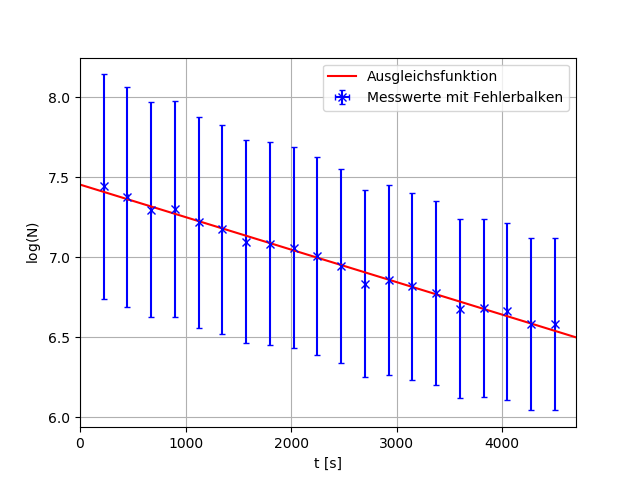
\includegraphics[scale=0.7]{Auswertung/Indium.png}
    \caption{Zerfall von Indium.}
    \label{fig:Indium}
\end{figure}
Für die Regression ergeben sich folgende Parameter:
\begin{gather*}
	m = -0.0002\pm 2.4\cdot10^{-11} \frac{1}{\text{s}}\\
	b = 7.45\pm0.00017
\end{gather*}
Nach Gleichung \ref{eq:3} ergibt sich nun für die Halbwertszeit
\begin{equation}
	T = \ln{\frac{2}{m}} = (3412.01 \pm 0.0004) \text{s}
\end{equation}
Nach Gleichung \ref{eq:3} kann zudem die Größe
\begin{gather*}
	\text{N}(0)(1-e^{-\increment t\lambda}) = 1725.07 \pm 0.30 \\
	=> \text{N}(0) = \frac{1725.07 \pm 0.30}{(1-e^{-\increment t\lambda})} = 2906.95 \pm 0.51
\end{gather*} 
bestimmt werden. Hierbei handelt es sich um die Isotopanzahl zu Beginn des Zerfalls.

\subsection{Silber}
Das Isotop $Ag^{108}$ und $Ag^{10}$ wird nun untersucht. Bei dem Zerfall werden folgende Werte gemessen (Tab. \ref{tab:2}).
Die Fehler ergeben sich nach Gleichung \ref{eq:fehler}.

\begin{table}
    \centering
\caption{Messwerte von Ag.}
\begin{minipage}{0.2\textwidth}
\label{tab:2}
    \centering
	\begin{tabular}{c|c|c}
		\toprule
		{$t / s$} & {$N$}&{$\sqrt{N}$}\\
		\hline
        \midrule
	9&70&8.37\\
	18&61&7.81\\
	27&50&7.07\\
	36&54&7.35\\
	45&35&5.92\\
	54&23&4.80\\
	63&24&4.90\\
	72&20&4.47\\
	81&19&4.36\\
	90&15&3.87\\
	99&19&4.36\\
	108&17&4.12\\
	117&18&4.24\\
	126&22&4.69\\
	135&19&4.36\\
	144&11&3.32\\
	153&16&4.00\\
	162&6&2.45\\
	171&8&2.83\\
	180&10&3.16\\
	189&5&2.24\\
	198&9&3.00\\
	207&13&3.61\\
	216&12&3.46\\
	225&7&2.65\\
	\bottomrule 
	\end{tabular}
\end{minipage}
\begin{minipage}{0.2\textwidth}
    \centering
	\begin{tabular}{c|c|c}
		\toprule
		{$t / s$} & {$N$}&{$\sqrt{N}$}\\
		\hline
        \midrule
	234&10&3.16\\
	243&6&2.45\\
	252&7&2.65\\
	261&4&2.00\\
	270&8&2.83\\
	279&9&3.00\\
	288&9&3.00\\
	297&7&2.65\\
	306&7&2.65\\
	315&4&2.00\\
	324&11&3.32\\
	333&6&2.45\\
	342&6&2.45\\
	351&8&2.83\\
	360&4&2.00\\
	369&5&2.24\\
	378&12&3.46\\
	387&4&2.00\\
	396&5&2.24\\
	405&6&2.45\\
	414&3&1.73\\
	423&2&1.41\\
	432&2&1.41\\
	441&6&2.45\\
	450&5&2.23\\
	\bottomrule 
	\end{tabular}
\end{minipage}
\end{table}

Die Werte aus Tabelle \ref{tab:2} sind in Abbildung \ref{fig:Silber} abgebildet.
\begin{figure}[H]
    \centering
    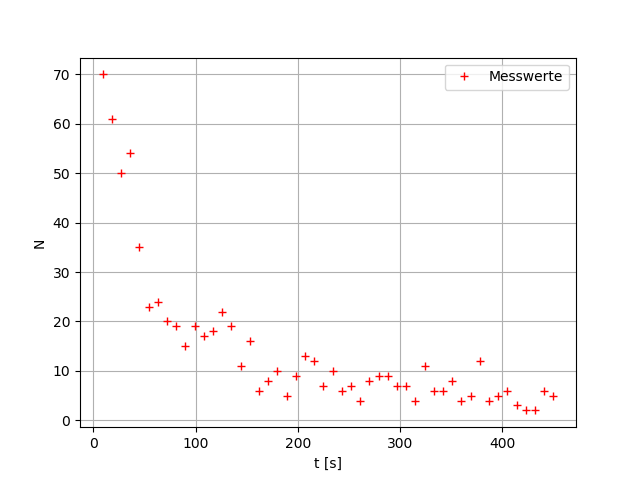
\includegraphics[scale=0.7]{Auswertung/Silber_alle.png}
    \caption{Zerfall von Silber.}
    \label{fig:Silber}
\end{figure}
Aus diesem Zerfall wird nun zunächst der langlebige Zerfall von $Ag^{108}$ untersucht. Sobald der Zerfall aus Abbildung \ref{fig:Silber} linear verläuft, wird angenommen, dass nur noch der langlebige Zerfall stattfindet. Für diesen Zeitpunkt wird t* =117s gewählt. \\
Werden diese Daten halblogarithmisch nach Gleichung \ref{eq:4} aufgetragen und mithilfe von linearer Regression nach
\begin{equation*}
	y = m\cdot x+b
\end{equation*}
eine Ausgleichgerade eingetragen, so ergibt sich folgender Graph (Abb. \ref{fig:lang}).
\begin{figure}[H]
    \centering
    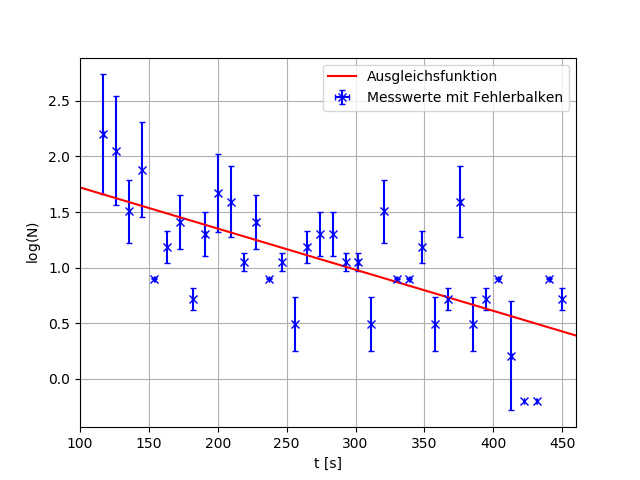
\includegraphics[scale=0.7]{Auswertung/Lang.png}
    \caption{Zerfall des langlebigen Silber-Isotops $Ag^{108}$.}
    \label{fig:lang}
\end{figure}
Für die Regression ergeben sich folgende Parameter:
\begin{gather*}
	m = -0.0053\pm 2.4\cdot10^{-7} \frac{1}{\text{s}}\\
	b = 2.605\pm0.014
\end{gather*}
Nach Gleichung \ref{eq:3} ergibt sich nun erneut für die Halbwertszeit
\begin{equation}
	T_1 = \ln{\frac{2}{m}} = (130.886 \pm 0.005) \text{s}
\end{equation}
Nach Gleichung \ref{eq:3} kann zudem die Größe
\begin{gather*}
	\text{N}(0)(1-e^{-\increment t\lambda}) = 13.46 \pm 0.19 \\
	=> \text{N}(0) = \frac{13.46 \pm 0.19}{(1-e^{-\increment t\lambda})} = 29.13 \pm 0.21
\end{gather*} bestimmt werden.
\\
Um nun den Zerfall des kurzlebigen Silber-Isotops $Ag^{110}$ zu bestimmen wird vom gesamten Zerfall der des langlebigen abgezogen:
\begin{equation*}
	N_{\increment t_s}(t) := N_{\increment t_\text{gesamt}} - N_{0,l} e^{-\lambda_l t} = N_{0,s} e^{-\lambda_s t}
\end{equation*} 
$N_{\increment t_s}(t)$ ist die Isotopanzahl des kurzlebigen Isotops nach einer Zeit $\increment t$, $N_{0l}$ ist die Isotopanzahl des langlebigen Isotops zu Beginn und  $\lambda_l$ ist die Zerfallskonstante des langlebigen Isotops und $N_{0,s}$ die Isotopanzahl des kurzlebigen Isotops zu Beginn.
Wird nun nur der Zeitraum bis 117 Sekunden betrachtet (Messwerte siehe \ref{tab:3}) und der Zerfall des langlebigen Isotops abgezogen, so ergibt sich folgender halblogarithmischer Graph mit Ausgleichsgrade anhand linearer Regression:
\begin{figure}[H]
    \centering
    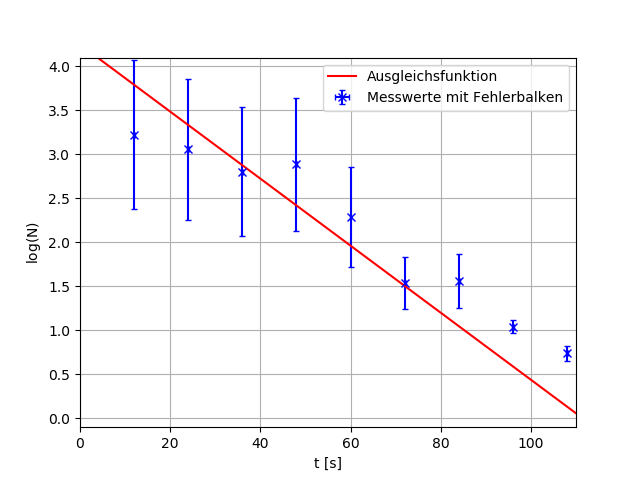
\includegraphics[scale=0.7]{Auswertung/kurz.png}
    \caption{Zerfall des kurzlebigen Silber-Isotops $Ag^{110}$.}
    \label{fig:kurz}
\end{figure}
\begin{table} [H]
	\centering
	\caption{Messwerte des kurzlebigen Isotops.}
	\label{tab:3}
	\sisetup{table-format=4.2}
	\begin{tabular}{c|c|c}
		\toprule
		{$t / \text{s}$}&{$N$}&{$\sqrt{N}$} \\
		\midrule
		9&61.53&7.84\\
		18&52.14&7.22\\
		27&40.74&6.38\\
		36&44.31&6.66\\
		45&24.86&4.99\\
		54&12.40&3.52\\
		63&12.91&3.59\\
		72&8.40&2.90\\
		81&6.87&2.62\\
		90&2.31&1.12\\
		99&5.72&2.39\\
		108&3.11&1.76\\
		117&3.47&1.86\\
		\bottomrule 
	\end{tabular}
\end{table} 
Die Fehler ergeben sich nach Gleichung \ref{eq:fehler}.
Für die Regression ergeben sich folgende Parameter:
\begin{gather*}
	m = -0.047\pm 7.0\cdot10^{-5} \frac{1}{\text{s}}\\
	b = 3.85\pm0.11
\end{gather*}
Nach Gleichung \ref{eq:3} ergibt sich nun erneut für die Halbwertszeit
\begin{equation}
	T_2 = \ln{\frac{2}{m}} = (14.697 \pm 0.022) \text{s}
\end{equation}
Nach Gleichung \ref{eq:3} kann zudem die Größe
\begin{gather*}
	\text{N}(0)(1-e^{-\increment t\lambda}) = 47 \pm 5 \\
	=> \text{N}(0) = \frac{47 \pm 5}{(1-e^{-\increment t\lambda})} = 51.77 \pm 5.51
\end{gather*}
bestimmt werden.
\begin{figure}[H]
    \centering
    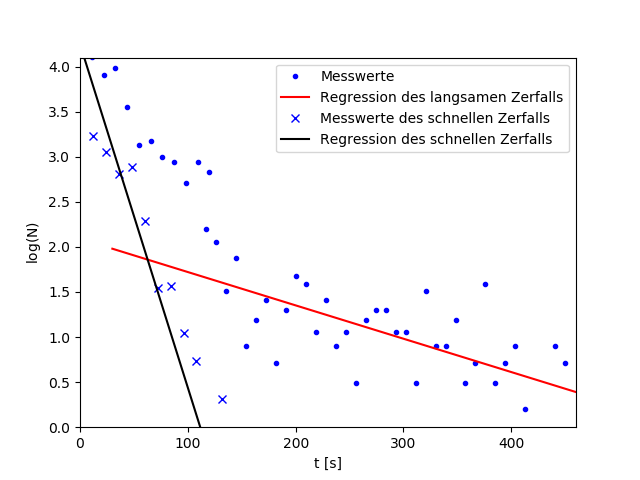
\includegraphics[scale=0.7]{Auswertung/Sum.png}
    \caption{Summenkurve von Silber.}
    \label{fig:sum}
\end{figure}
Um zum Schluss die Ungleichung
\begin{equation*}
	N_{\increment, kurz}(t_i) << N_{\increment, lang}(t_i)
\end{equation*}
zu beweisen, werden die beiden Werte zum Zeitpunkt $t_i$ = 117s bestimmt (siehe oben).
Daraus folgt:
\begin{equation*}
	7.5 \pm 0.6 << 14.5 \pm 0.6 .
\end{equation*}
Somit ist die Ungleichung bestätigt.
	